%% ----------------------------------------------------------------
%% Analysis.tex
%% ---------------------------------------------------------------- 


\chapter{Purposive Social Network Analysis} \label{Chapter:Purposive Social Network Analysis}

A purposive social network is a broad and general concept that can be applied to many different social networks. At its core, it is a network with a specific goal and purpose where people come together to solve a particular problem.

For this research StackOverflow website is analyzed where programmers and developers ask questions and experts in the field answer them and solve the problem. In this analysis, the user asking and answering questions, voting the responses and commenting are the main entities of the social network. Their network ties are measured by their communication and interaction between them. The amount of their contribution is measured by the crowdsourcing where people give up votes or down votes to their posts and the badges they receive for their contribution.


\section{Network Linkage and Social Ties}

StackOverflow is not a typical social networking website per se as users cannot create an explicit friendship or follow other peopleÕs work, they cannot send private messages or form groups.

The social ties are form implicit by user interaction with each other through asking questions and answering them, voting on the posts and commenting on them. The communication network is studied to see the social ties of the individuals \cite{monge2003theories}.

\begin{table}[!htb]
  \centering
  \begin{tabular}{cc}
  \toprule
  \textbf{Post Type} & \textbf{Number}\\
  \midrule
   Questions & 3279233\\   \midrule
   Answers & 6578079\\   \midrule
   Registered Users & 1225580\\   \midrule
   Tags & 30408 \\   \midrule
   Unanswered Questions & 780535\\   \midrule
   Badges & 3454994\\   \midrule
   Votes & 26184363\\   \midrule
   Comments & 12526162\\ 
  \bottomrule
  \end{tabular}
  \caption{StackOverflow at glance as of June 2012}
  \label{Table:tabex}
\end{table}

As of June 2012, there are over one million registered users in StackOverflow and more than 3.2 millions questions asked by users. The questions are categorized using tags and individual users can subscribe to tags to receive daily email of all the question asked in the tag. There are more than 30 thousand tags associated with various questions and answers. Users have casted more than 26 million votes to mark the good questions and answers.

\begin{figure}[!htb]
  \centering
  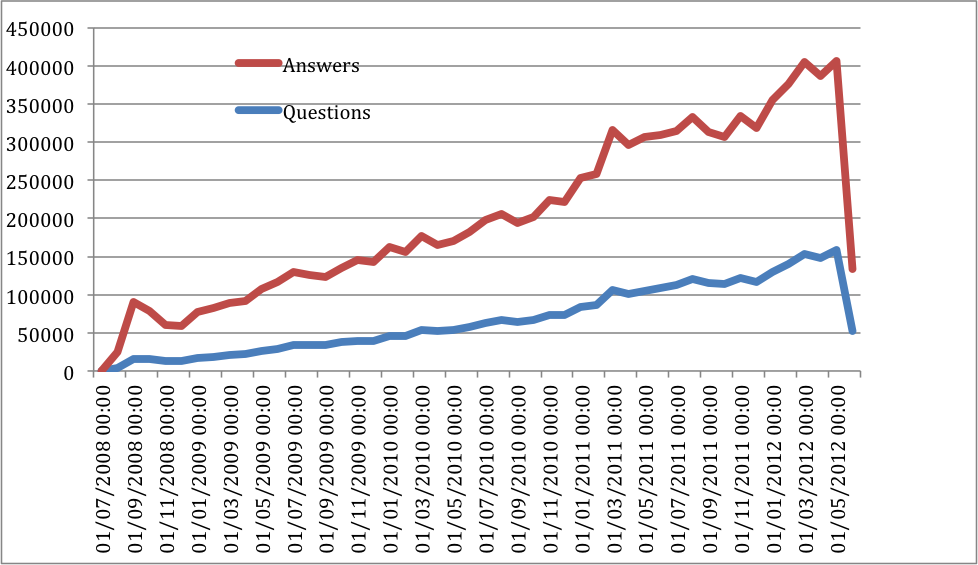
\includegraphics[width=15cm]{qa.png}
  \caption{Questions and answers posted per month on StackOverflow}
  \label{Figure:figex4a}
\end{figure}

The \fref{Figure:figex4a} shows the number of questions asked and answered by users each month. In the year 2012, each questions have on average 1.645 number of answers.

This community is made of programmers and their motivation is to solve the problem they had encountered and to provide answers to gain reputations. Thousands of questions and answers are posted everyday. The analysis of posts shows that the programmers prefer to ask the questions and answers on weekdays.

\begin{figure}[!htb]
  \centering
  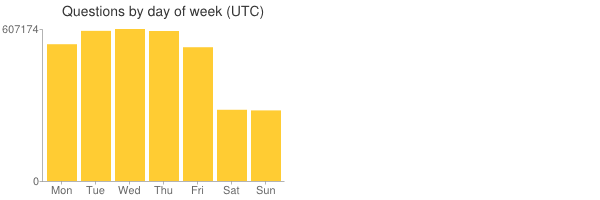
\includegraphics[width=15cm]{chart1.png}
  \caption{Questions posted by the day of week}
  \label{Figure:figex4b}
\end{figure}

Despite high user feedback and participation, 23.79\% of questions are not answered or the answers do not receive any up votes. On average a question receives 2.006 answers and .12\% of questions receives more than 15 answers.

\begin{figure}[!htb]
  \centering
  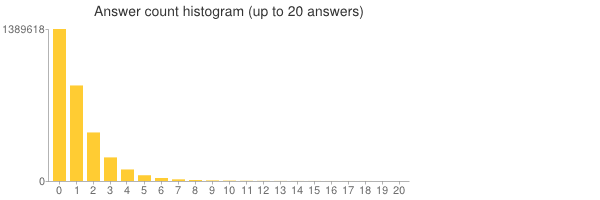
\includegraphics[width=15cm]{chart2.png}
  \caption{Answer count to the questions}
  \label{Figure:figex4c}
\end{figure}

The questions are answers are provided with tags to categorize and arrange for easy search and discovery. The entire website is categorized using the tags and the list of most popular tags are shown in the table. The figure shows the weekly use of the popular tags. The number of questions asked for each tags also provides an insight on the popular language used by developers at the time.

\begin{table}[!htb]
  \centering
  \begin{tabular}{cc}
  \toprule
  \textbf{Tags} & \textbf{Number of instance}\\  \midrule
   C\# & 370074 \\ \midrule
   JAVA &  315488 \\ \midrule
   PHP & 293755 \\ \midrule
   JavaScript & 278592 \\ \midrule
   Android & 244791 \\
  \bottomrule
  \end{tabular}
  \caption{Five most popular tags and its instances}
  \label{Table:tabex2}
\end{table}

\begin{figure}[!htb]
  \centering
  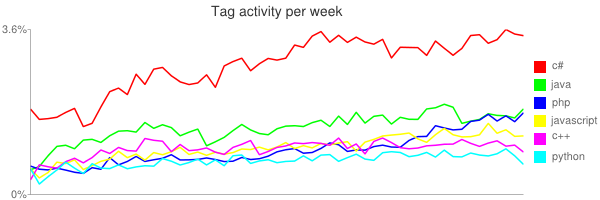
\includegraphics[width=15cm]{chart3.png}
  \caption{Tag trends per week of most popular tags}
  \label{Figure:figex4d}
\end{figure}

The analysis of questions shows that each question has between one to five tags associated with it. Most questions (70.30\%) have 2 to 4 tags associated with it. The relationship between the tags shows the overlapping of networks and how it is tied with one another.

\cite{Eberhardt2012} provided an interactive graph in his website to show the relationships between the most popular tags and how closely they are related to each other. In the following graph each segment size is directly proportional to the number of instance it is used and the connection between the tags indicate the times they have been used together in a question. The thickness of the connection shows the strength of the relations. The segment is colour coded by the frequency of connections, red segments are strongly connected and blue segments are weakly connected.

\begin{figure}[!htb]
  \centering
  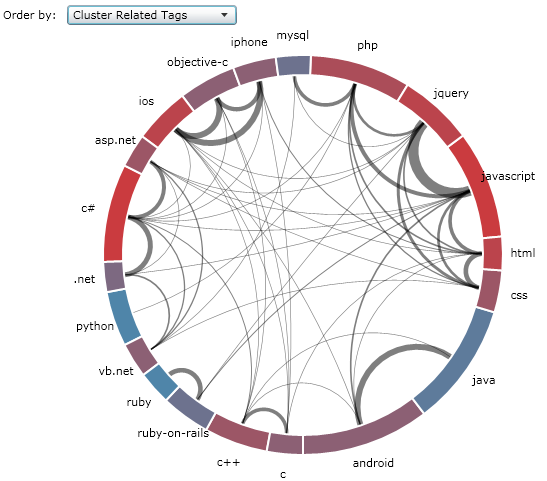
\includegraphics[width=11cm]{graph1.png}
  \caption{Related tags clustered together}
  \label{Figure:figex4e}
\end{figure}

\begin{figure}[!htb]
  \centering
  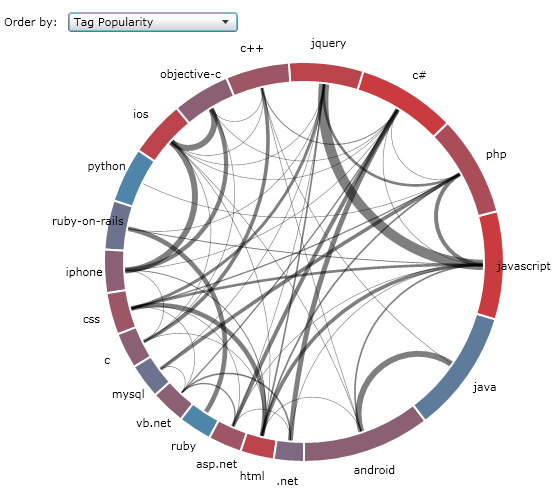
\includegraphics[width=11cm]{graph2.png}
  \caption{Popular tags clustered together}
  \label{Figure:figex4f}
\end{figure}

The clustering of the tags shows the relationship between the tags and technologies. The two popular tags JAVA and Android are closely related to each other but are scarcely joined with other tags. The strongest relationship is between jQuery and JavaScript because the overlapping framework of the two programming languages. C, C++ and C\# are also a closely related groups as well as iOS, Objective-C and iPhone. However, sometimes Objective-C is also tagged with C, C++ and C\#, if by mistake or deliberately can be argued.
There is a large cluster of connected web development languages, CSS, HTML, JavaScript and jQuery, indicating the close knit use of these technologies in development of website and web applications. The interesting thing is the relationship between the scripting langue PHP and Python, they are popular tags but are sparsely connected with other tags and are weakly linked with database related tags.


\section{Role of Individual Actors}

Users who contribute to the website are the main actors of this purposive social network. There are more than 1.2 million registered users in StackOverflow and they ask the questions, answer it, vote it and moderate the community. The users are not directly linked to each other to create relationships; in this network the relationship is formed by their interaction and their contribution. The user behaviour, their motivation to use the website and incentive to contribute is described below.

Despite the high content generation by the users, 56.02\% do not interact or contribute to the website, they have 1 reputation point that they receive while joining the website.

\begin{figure}[!htb]
  \centering
  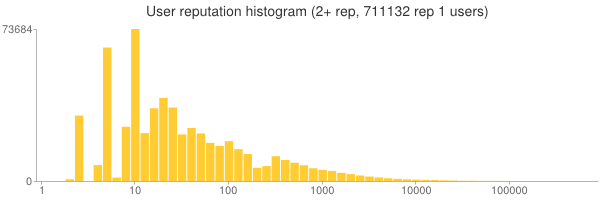
\includegraphics[width=15cm]{chart4.png}
  \caption{User reputation histogram}
  \label{Figure:figex4g}
\end{figure}

\begin{table}[!htb]
  \centering
  \begin{tabular}{cc}
  \toprule
  \textbf{Reputation} & \textbf{Number of users}\\  \midrule
  1 & 669554\\ \midrule
  2-10 & 126235\\ \midrule
  11-100 & 295389\\ \midrule
  101-1000 & 3161130\\  \midrule
  1001-10000 & 170993\\ \midrule
  10001-20000 & 1437\\ \midrule
  20001-100000 & 895\\ \midrule
  100001-200000 & 49\\ \midrule
  less than 200000 & 11\\
  \bottomrule
  \end{tabular}
  \caption{Number of users with reputations}
  \label{Table:tabex3}
\end{table}

As \tref{Table:tabex3} shows, there are 669554 users with 1 reputation point and one user with 452951 reputation points. The distribution of the users reputation shows that more than half of the users are lurkers and the elite users with the most reputation points are the editors and moderators of the community and are considered the expert in their field.

The reputation of the user has a direct correlation with the trust in the community. StackOverflow has designed an excellent reward program to motivate and incentivize the users to contribute and gain more reputations and badges.

Currently, there are 77 different types of badges given to the user based on their contribution. There are badges given to the user who asks questions with 1 reputation point (Student), to the user who edits the answers to make posts better (Editor) and to even an active user for a year (Yearling). This type of virtual acknowledgement of efforts encourage the user to participate and contribute to the website.

The other method that encourages the users to participate is the promptness of the response. The asker prefers to receive information sooner rather than later, and will stop the process when satisfied with the cumulative value of the posted information. The analysis of the posts shows that half of the questions get an answer within an hour of the posting and within a day the questions receives an accepted answer. When the answers are delayed, the questioners look for alternative websites to get a response.

\begin{figure}[!htb]
  \centering
  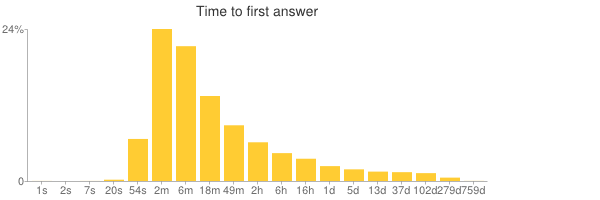
\includegraphics[width=15cm]{chart5.png}
  \caption{Time to receive the first answer}
  \label{Figure:figex4h}
\end{figure}

\begin{figure}[!htb]
  \centering
  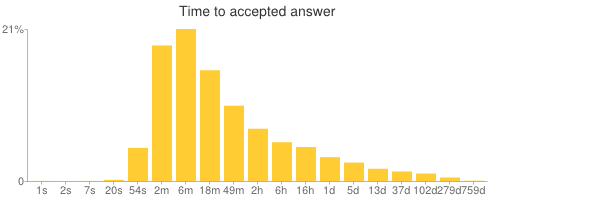
\includegraphics[width=15cm]{chart6.png}
  \caption{Time to get the accepted answer}
  \label{Figure:figex4i}
\end{figure}


\section{Incentive Design}

The StackOverflow website uses a game theoretic model to encourage user participation and activity. Participation is encouraged through an elaborate point system and users also receive badges for participation. Also, the top contributor and user with highest reputation are featured on the question page, giving the user more visibility and acknowledgement of the userÕs expertise. This encourages participants to accumulate more points and contribute to get recognition.

When an answer is votes up, the user gains 10 reputations and 5 points when the question is voted up. When an answer is accepted the user receives 15 points and there is also negative point system, a user looses 2 reputation point when a question or an answer is voted down. This keeps the spamming in check and repeated questions and answers are avoided.

The system also encourages users to participate as the higher reputation points gain more privileges. When a user has 15 reputation points, only then they can up vote and 50 points allows users to comment. To stop harassment and spam, user requires 125 reputation points to vote down and it costs the user 1 reputation point. The incentive model is thorough and higher reputation points open more gates for users to interact and contribute and be acknowledged as the expert in their field.


\section{Quality Control}

The community thrives because of the high quality of content and it is possible by the userÕs action and moderation. Users vote up the good questions and answers and vote down the bad quality content or repeated posts. There is more than 6 million votes casted in the website and the user with enough reputations are allowed to cast 40 votes per day.

\begin{figure}[!htb]
  \centering
  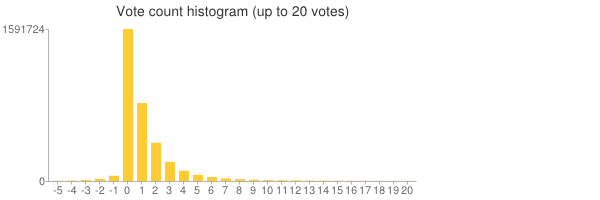
\includegraphics[width=15cm]{chart7.png}
  \caption{Vote count histogram}
  \label{Figure:figex4j}
\end{figure}

\begin{table}[!htb]
  \centering
  \begin{tabular}{cc}
  \toprule
  \textbf{Vote} & \textbf{Vote Count}\\  \midrule
  less than 20 & 25\\  \midrule
  0 & 504754\\  \midrule
  1-10 & 7802690\\  \midrule
  11-100 & 718650\\  \midrule
  101-1000 & 6460\\  \midrule
  1000-5000 &11\\
  \bottomrule
  \end{tabular}
  \caption{QuestionsÕ votes count}
  \label{Table:tabex4}
\end{table}

The analysis of the questions and votes shows that every question receives 3.06 votes on average. One question received negative 115 votes and the highest vote received to a question is 2499. Similar analysis of answers and their votes shows that, on average an answer receives 0.99 votes and the lowest vote to an answer is negative 57 and the highest vote is 4432.


\section{Linked Data Graph}




\section{Discourse Analysis}